\documentclass{ctexart}

\usepackage{amsmath}

\usepackage{amsthm}

\usepackage{amssymb}

\usepackage{mathabx}

\usepackage{bm}

\usepackage{graphicx}

\usepackage{listings}
\lstset{
basicstyle=\scriptsize
}

\usepackage{caption}

\begin{document}

\title{统计中的计算方法 \\ 第一次作业}

\author{于慧倩 \\ 14300180118}

\date{2017年4月}


\maketitle

\newpage

\begin{enumerate}

%第一题
\item
假设\(\bm{X}=(X_1,X_2,\dots,X_n)\)是\(n\)个来自于三个二元正态分布的混合分布的独立样本,推导出用EM方法估计三个二元正态分布参数的迭代步骤。

二元正态分布的概率密度函数\(f\)为
\[ f(x_1,x_2)=\frac{1}{\sqrt{(2 \pi)^2|\bm{\Sigma}|}}\exp(-\frac{1}{2}(\bm{x}-\bm{\mu})^T \bm{\Sigma}^{-1} (\bm{x}-\bm{\mu}))\]

令\(\bm{z}=(z_1,z_2,\dots,z_n)\)代表\(\bm{x}\)属于哪一个独立分布,即:
\[
x_i|(z_i=1) \sim N(\bm{x}_1,\bm{\sigma_1}),
x_i|(z_i=2) \sim N(\bm{x}_2,\bm{\sigma}_1),
x_i|(z_i=3) \sim N(\bm{x}_3,\bm{\sigma}_3)\]

有
\[
P(z_i=1)=\tau_1,P(z_i=2)=\tau_2,P(z_i=3)=\tau_3\]
其中
\[\tau_1+\tau_2+\tau_3=1\]

令\(z_{ij}=1\)表示第\(i\)个样本属于第\(j\)个分布。
则有似然函数为
\[ L( \theta |\bm{x},\bm{z})=P(\bm{x},\bm{z}|\theta)= \prod_{i=1}^n \prod_{j=1}^3 (\tau_j f( \bm{x}_i;\bm{\mu}_j,\bm{\Sigma}_i))^{z_{ij}} \]

那么有log似然函数:
\[
\log L(\theta|\bm{x},\bm{z})=\sum_{i=1}^n \sum_{j=1}^3 z_{ij} [ \log{ \tau_j} - \frac{1}{2} \log|\bm{\Sigma}_j |]-\frac{1}{2}(\bm{x}_i-\bm{\mu}_j)^T \bm{\Sigma}_j^{-1} (\bm{x}_i-\bm{\mu}_j)-\log(2 \pi)]\]

\begin{enumerate}


\item E-step:
\begin{eqnarray*}
Q(\theta | \theta^{(t)})&=&E(\log L(\theta|\bm{x},\bm{z})) \\
&=&E(\sum_{i=1}^n \sum_{j=1}^3 z_{ij} [ \log{ \tau_j} - \frac{1}{2} \log|\bm{\Sigma}_j |]-\frac{1}{2}(\bm{x}_i-\bm{\mu}_j)^T \bm{\Sigma}_j^{-1} (\bm{x}_i-\bm{\mu}_j)-\log(2 \pi)])\\
&=& \sum_{i=1}^n \sum_{j=1}^3 T_{ij}^{(t)} [ \log{ \tau_j} - \frac{1}{2} \log|\bm{\Sigma}_j |]-\frac{1}{2}(\bm{x}_i-\bm{\mu}_j)^T \bm{\Sigma}_j^{-1} (\bm{x}_i-\bm{\mu}_j)-\log(2 \pi)]
\end{eqnarray*}

其中
\[
T_{ij}^{(t)} =P(z_{ij}=1|X_i=\bm{x}_i;\theta^{(t)})=\frac{ \tau^{(t)}_j  f( \bm{x}_i;\bm{\mu}_j^{(t)},\bm{\Sigma}_j^{(t)})}{\displaystyle \sum_{j=1}^3\tau^{(t)}_j  f( \bm{x}_i;\bm{\mu}_j^{(t)},\bm{\Sigma}_j^{(t)})}\]

 \item M-step:
 
 \begin{enumerate}
 \item 对于\(\tau_j\)利用MLE方法进行估计:

\begin{eqnarray*}
\tau^{(t+1)} &=& \mathop{\text{arg} \max}_{\tau} Q(\theta|\theta^{(t)}) \\
&=& \mathop{\text{arg} \max}_{\tau} \{ \sum_{j=1}^3  [\sum_{i=1}^n T_{i,j}^{(t)}]\log \tau_j    \}
\end{eqnarray*}

利用MLE方法与\(\tau_1+\tau_2+\tau_3=1\),令\(\tau_3=1-\tau_1-\tau_2\),得到对\(\tau_1\)求导式子并令其为零:
\[ \frac{\displaystyle \sum_{i=1}^n T_{1,i}^{(t)}}{\tau_1}-\frac{\displaystyle \sum_{i=1}^n T_{3,i}^{(t)}}{1-\tau_1-\tau_2} =0\]

另对\(\tau_2\)求导,可以得到\(\tau_j\)之间的关系式:
\[
\tau_1= \frac{\displaystyle \sum_{i=1}^n T_{1,i}^{(t)}} {\displaystyle \sum_{i=1}^n T_{3,i}^{(t)}} \tau_3\]
\[
\tau_2= \frac{\displaystyle \sum_{i=1}^n T_{2,i}^{(t)}} {\displaystyle \sum_{i=1}^n T_{3,i}^{(t)}} \tau_3\]

并且有\(\tau_1+\tau_2+\tau_3=1= \frac  {\displaystyle \sum_{i=1}^n (T_{1,i}^{(t)}+T_{2,i}^{(t)}+T_{3,i}^{(t)})}
 {\displaystyle \sum_{i=1}^n (T_{1,i}^{(t)}+T_{2,i}^{(t)}+T_{3,i}^{(t)})}
\)所以得到:

\[ \tau_j^{(t+1)}= \frac {\displaystyle \sum_{i=1}^n T_{j,i}^{(t)}} {\displaystyle \sum_{i=1}^n (T_{1,i}^{(t)}+T_{2,i}^{(t)}+T_{3,i}^{(t)})}
\]

\item
对于\((\mu_j,\bm{\Sigma}_j)\)同样利用MLE方法进行估计:
\begin{eqnarray*}
(\bm{\mu}_1^{(t+1)},\bm{\Sigma}_1{(t+1)}) &=& \mathop{\text{arg} \max}_{\bm{\mu}_1,\bm{\Sigma}_1} Q(\theta | \theta^{(t)}) \\
&=& \mathop{\text{arg} \max}_{\mu_1,\bm{\Sigma}_1}  \sum_{i=1}^n T_{1,i}^{(t)} \{ -\frac{1}{2} \log |\bm{\Sigma}_1| -\frac{1}{2} (\bm{x}_i-\bm{\mu}_1)^T\bm{\Sigma}_1^{-1}  (\bm{x}_i -\bm{\mu}_1) \}
\end{eqnarray*}

对于\(\mu_1\)求导令其为0,得到:
\[\sum_{i=1}^n T_{1,i}^{(t)} \{ \bm{\Sigma}^{-1}(\bm{x}_i-\bm{\mu}_1)=0\]

进一步得到:

\[
\bm{\mu}_1^{(t+1)}= \frac{ \displaystyle \sum_{i=1}^n T_{1,i}^{(t)} \bm{x}_i  }{\displaystyle \sum_{i=1}^n T_{1,i}^{(t)}}\]

另对\(\bm{\Sigma}_1\)求导,得到:
\[
\sum_{i=1}^n T_{1,i}^{(t)} [ \bm{\Sigma} -(\bm{x}_i-\bm{\mu}_1)(\bm{x}_i-\bm{\mu}_1)^T ] =0\]

\[
\bm{\Sigma}_1^{(t+1)}=\frac{\displaystyle \sum_{i=1}^n T_{1,i}^{(t)} (\bm{x}_i-\bm{\mu}_1^{(t+1)})(\bm{x}_i-\bm{\mu}_1^{(t+1)})^T}{\displaystyle \sum_{i=1}^n T_{1,i}^{(t)}}\]
同理由对称性得到:
\[
\bm{\mu}_2^{(t+1)}= \frac{ \displaystyle \sum_{i=1}^n T_{2,i}^{(t)} \bm{x}_i  }{\displaystyle \sum_{i=1}^n T_{2,i}^{(t)}}\]
\[
\bm{\Sigma}_2^{(t+1)}=\frac{\displaystyle \sum_{i=1}^n T_{2,i}^{(t)} (\bm{x}_i-\bm{\mu}_2^{(t+1)})(\bm{x}_i-\bm{\mu}_2^{(t+1)})^T}{\displaystyle \sum_{i=1}^n T_{2,i}^{(t)}}\]
\[
\bm{\mu}_3^{(t+1)}= \frac{ \displaystyle \sum_{i=1}^n T_{3,i}^{(t)} \bm{x}_i  }{\displaystyle \sum_{i=1}^n T_{3,i}^{(t)}}\]
\[
\bm{\Sigma}_3^{(t+1)}=\frac{\displaystyle \sum_{i=1}^n T_{3,i}^{(t)} (\bm{x}_i-\bm{\mu}_3^{(t+1)})(\bm{x}_i-\bm{\mu}_3^{(t+1)})^T}{\displaystyle \sum_{i=1}^n T_{3,i}^{(t)}}\]

\end{enumerate}

\end{enumerate}

\item
对数据Data1.csv用1.中方法进行估计参数。

\centerline{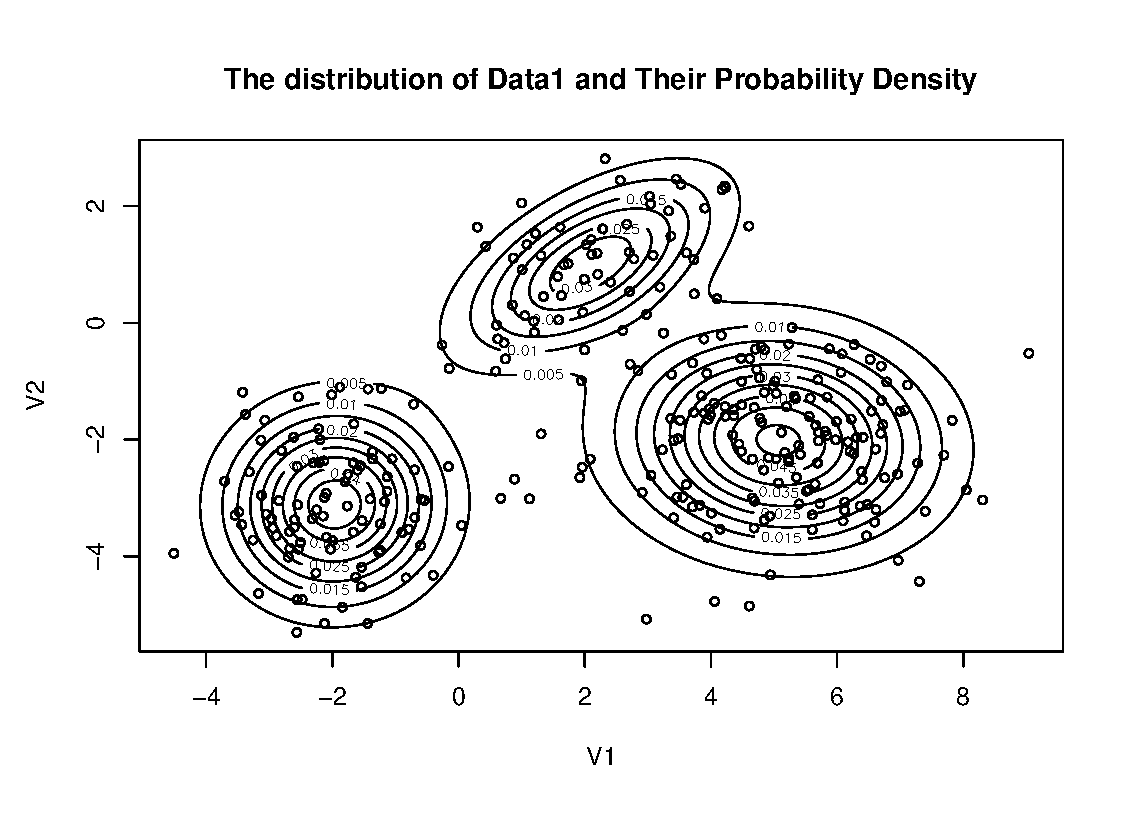
\includegraphics[width=5.5in]{2.eps}}

按照1.的方法进行估计迭代,在选取迭代初值的时候,将全部数据平均分为三份,分别计算它们的期望和协方差矩阵。迭代获得最终分布如图,三个二元正态分布的参数如下表:

\centerline{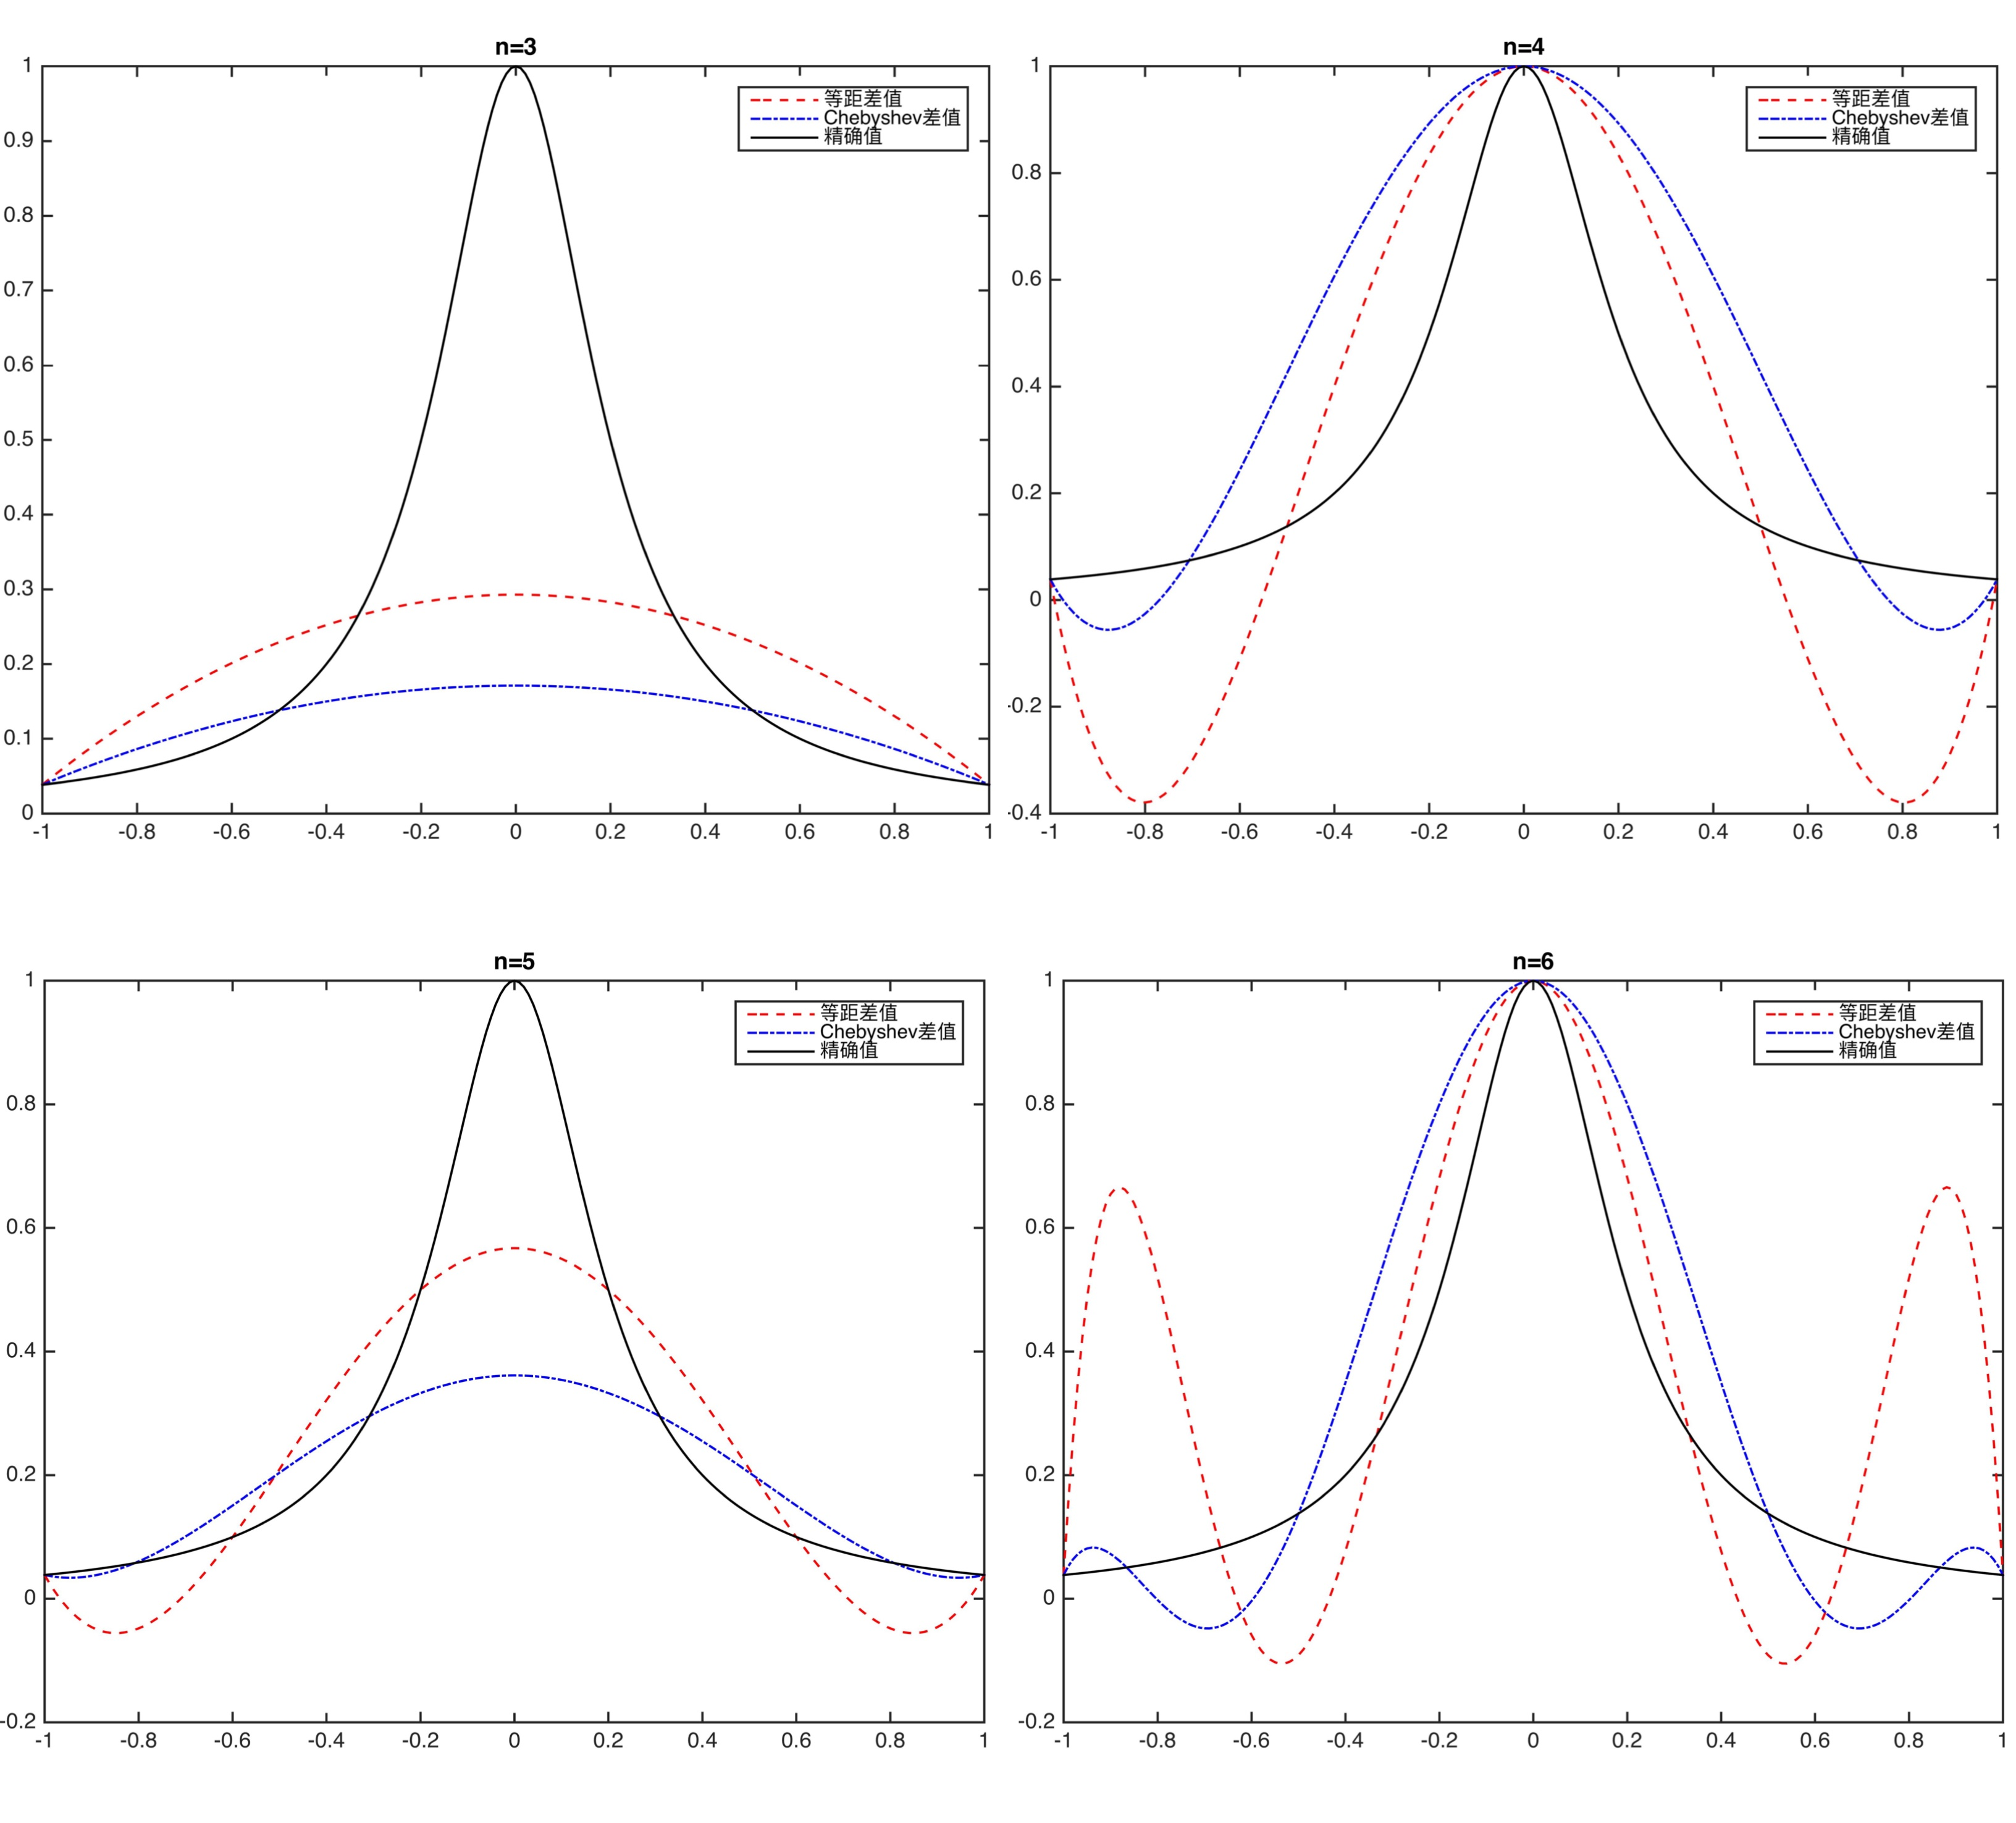
\includegraphics[width=5in]{1.jpg}}




%第三题
\item
一组随机抽样中随机变量\(\xi\)取值为0,1,2,3,4,5,6,观察到\(\xi\)取0,1,2,3,4,5,6的次数为\(n_0,n_1,n_2,n_3,n_4,n_5,n_6\)。假设随机变量实际服从两个总体的混合分布:总体A:以概率\(p\),随机变量取值为0;总体B:以概率\(1-p\),随机变量服从均值为\(\lambda\)的泊松分布;设计EM算法估计\(p\)和\(\lambda\)。


  我们有\(\xi\)取值\((0,1,2,3,4,5,6)\)的概率为\(
p+(1-p) e^{-\lambda} ,
(1-p) \lambda e^{-\lambda}, 
(1-p)\frac{\lambda^2 e^{-\lambda}}{2}, 
(1-p)\frac{\lambda^3 e^{-\lambda}}{3!} , 
(1-p)\frac{\lambda^4 e^{-\lambda}}{4!}, 
(1-p)\frac{\lambda^5 e^{-\lambda}}{5!},
(1-p)\frac{\lambda^6 e^{-\lambda}}{6!}  
\)。我们观察到的数据为\(\bm{\xi}=(n_0,n_1,n_2,n_3,n_4,n_5,n_6)^T\)。未知参数向量\(\theta=(\lambda,p)^T\)。

有似然函数:
\[L(\theta)=(p+(1-p)e^{-\lambda})^{n_0} \prod_{i=1}^6 [(1-p^{(t)})\frac{\lambda^{(t)^i} e^{-\lambda^{(t)}}}{i!}]^{n_i}\prod_{i \geq 7}^{\infty} 1\]

除去常数后的log似然函数为
\[
\log L(\theta)=n_0 \log(p+(1-p) e^{-\lambda})+\sum_{i=1}^6 n_i\log((1-p)\lambda^ie^{-\lambda})\]



令\(n_0=n_{0A}+n_{0B}\),其中\(n_{0A},n_{0B}\)分别表示\(\xi\)取值为0且属于A分布的个数与\(\xi\)取值为0且属于B分布的个数。

则有似然函数
\[L(\theta | \theta^{(t)})=p^{(t)^{n_{0A}^{(t)}} }[(1-p^{(t)})e^{-\lambda^{(t)}}]^{n_{0B}^{(t)}}  \prod_{i=1}^6 [(1-p^{(t)})\frac{\lambda^{(t)^i} e^{-\lambda^{(t)}}}{i!}]^{n_i}\]





则去除常数的log似然函数为
\[\log L(\theta) =n_{0A} \log p +n_{0B}[\log(1-p)-\lambda]+\sum_{i=1}^6 n_i [\log(1-p)+i \log( \lambda)-\lambda] \]

\begin{enumerate}
\item E-step:
\begin{eqnarray*}
Q(\theta|\theta^{(t)})&=&E(\log L(\theta;\bm{\xi})) \\
&=& E\{ n_{0A} \log p +n_{0B}[\log(1-p)-\lambda] + \sum_{i=1}^6 n_i[\log (1-p)+i \log(\lambda)-\lambda]\}\\
&=& n_{0A}^{(t)} \log p +n_{0B}^{(t)}  [\log(1-p)-\lambda] +\sum_{i=1}^6 n_i[ \log (1-p)+i \log(\lambda)-\lambda]
\end{eqnarray*}

有概率如下:
\[P(\xi \in A| \xi=0)=\frac{p}{p+(1-p)e^{-\lambda}},
P(\xi \in B| \xi=0)=\frac{(1-p)e^{-\lambda}}{p+(1-p)e^{-\lambda}}\]

且 
\[n_{0A}^{(t)}=P(\xi \in A| \xi=0)n_0=\frac{p^{(t)}}{p^{(t)}+(1-p^{(t)})e^{-\lambda^{(t)}}}n_0\]
\[n_{0b}^{(t)}=P(\xi \in B| \xi=0)n_0=\frac{(1-p^{(t)})e^{-\lambda}}{p^{(t)}+(1-p^{(t)})e^{-\lambda^{(t)}}}n_0\]

\item M-step:

\begin{enumerate}
\item 对\(p\)进行估计:
\begin{eqnarray*}
p^{(t+1)}&=&\mathop{\text{arg} \max}_{p} Q(\theta|\theta^{(t)})\\
&=& \mathop{\text{arg} \max}_{p}  \{n_{0A}^{(t)} \log p +n_{0B}^{(t)}  \log(1-p) + \sum_{i=1}^6 n_i \log (1-p) \}\\
\end{eqnarray*}

等号右端对\(p\)求导,令其为零得到:
\[
p^{(t+1)}=\frac{n_{0A}^{(t)}}{n}\]

\item 对\(\lambda\)进行估计:
\begin{eqnarray*}
\lambda^{(t+1)}&=&\mathop{\text{arg} \max}_{\lambda}Q(\theta|\theta^{(t)})\\
&=&n_{0B}^{(t)} (-\lambda)+\sum_{i=1}^6 n_i[i\log \lambda-\lambda] 
\end{eqnarray*}



\[
\lambda^{(t+1)}= \frac{\displaystyle \sum_{i=1}^6 i*n_i}{n-n_{0A}^{(t)}}\]

\end{enumerate}
 
\end{enumerate}

\item
对数据Data2.csv用3.中方法进行估计参数。

\centerline{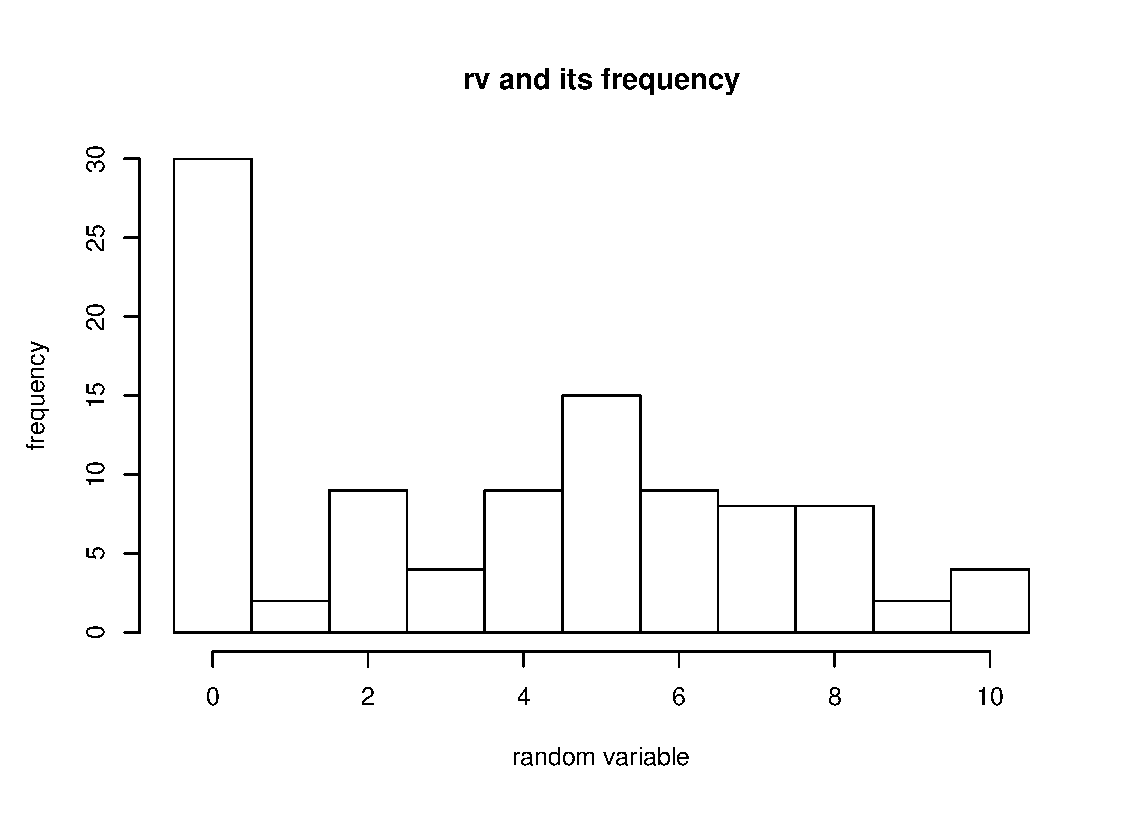
\includegraphics[width=5.5in]{4.eps}}

将所有数据的均值作为\(\lambda\)初始值,将\(\xi = 0\)的频率作为\(p\)初始值,迭代得到最终结果:
\[ p = 0.2965968 \]
 \[\lambda = 5.331224\]
















\end{enumerate}
\end{document}